
\section{MACRON}\label{appendix:macron}
\subsection{Contexto}

O exemplo a seguir baseia-se no contexto apresentado na Seção \ref{subsec:macron}. Em resumo, um agente \textit{QueryManagerAgent} deseja obter um serviço, especificamente, o serviço \textit{Get Online Reviews}. O diagrama apresentado na Seção \ref{fig:macron_example} é base da implementação deste contexto.

\subsection{Preparação do ambiente}\label{subsec:preparacao_ambiente_eclipse}

Devem ser seguidos os mesmos passos da Seção \ref{subsec:preparacao_ambiente_eclipse}, porém, deve-se optar pelo \textit{package} \textit{\textbf{macron}}.

\subsection{Classe \textit{Main}}

A \textit{Main}, nesta implementação, apenas recebe as requisições dos \textit{Query Manager Agents}, e, no caso, apenas do \textit{QueryManagerAgent}. Quando o serviço que este busca está disponível, é delegado que seja executado.

\begin{lstlisting}
package macron;

public class Main {

	public static void main(String[] args) {	
		QueryManagerAgent queryManager = new QueryManagerAgent();
		Boolean isServiceAvailable;
		
		//QueryManager wants to retrieve all online reviews about some product,
		isServiceAvailable = queryManager.findFunctionalManager("Get Online Reviews");
		
		//The query can only occur if there is an agent that can execute it.
		if (isServiceAvailable == true) {
			queryManager.executeQuery();
		} 
	}
}
\end{lstlisting}

\subsection{Classe \textit{QueryManagerAgent}}

O \textit{QueryManagerAgent} consulta o \textit{OrganizationChartManagerAgent} para verificar se há algum agente que ofereça o serviço que busca, através da função \textit{findFunctionalManager(String requestedService)}. Também delega ao \textit{OrganizationChartManagerAgent} que controle a execução do serviço quando o mesmo é encontrado e está disponível, através da função \textit{executeQuery()}. 

\begin{lstlisting}
package macron;

public class QueryManagerAgent {

	String requestedService;
	OrganizationChartManagerAgent ocmAgent = new OrganizationChartManagerAgent();
	
	//Verify if there is any functional manager that can offer the requested service
	protected Boolean findFunctionalManager(String requestedService) {
		return this.ocmAgent.findFunctionalManager(requestedService);
	}
	
	//Delegates ocmAgent to control the query execution
	protected void executeQuery() {
		this.ocmAgent.ordenateServiceExecution();
	}
}
\end{lstlisting}

\subsection{Classe \textit{OrganizationalChartManagerAgent}}

O \textit{OrganizationalChartManagerAgent} procura \textit{Functional Managers} através do método \textit{findFunctionalManager(String requestedService)} cujas \textit{Functional Units} possam desempenhar o serviço \textit{Get Online Reviews}. Sua principal função é conhecer os gerentes funcionais, sua disponibilidade, suas capacidades, e assim pode ser consultado pelo \textit{Query Manager} a qualquer instante. 

\begin{lstlisting}
package macron;

import java.util.HashMap;
import java.util.Map;

public class OrganizationChartManagerAgent {
	
	//OCM known agents
	private FunctionalManager1Agent fm1Agent = new FunctionalManager1Agent();
	private FunctionalManager2Agent fm2Agent = new FunctionalManager2Agent();
	
	//All services this agents offers
	private Map allServices = new HashMap<>();
	
	//The agent localized to execute the service to the query manager
	private String functionalManagerLocalized;
	
	public OrganizationChartManagerAgent() {
		this.allServices.put(fm1Agent.getService(), fm1Agent.getName());
		this.allServices.put(fm2Agent.getService(), fm2Agent.getName());
	}
	
	protected Boolean findFunctionalManager(String requestedService) {
		this.functionalManagerLocalized = (String) this.allServices.get(requestedService);
		if (this.functionalManagerLocalized != null) {
			System.out.println("The requested service can be executed by the " + this.functionalManagerLocalized + ".");
			return true;
		} else {
			System.out.println("The requested service has no functional manager that can do it.");
			return false;
		}
	}
	
	protected void ordenateServiceExecution() {
		if (this.functionalManagerLocalized == "Functional Manager 1") {
			this.fm1Agent.executeService();
		} else if (this.functionalManagerLocalized == "Functional Manager 2") {
			this.fm2Agent.executeService();
		}
	}

}
\end{lstlisting}
 
\subsection{Classe \textit{FunctionalManager1Agent}}

A pedido do \textit{QueryManagerAgent}, o \textit{FunctionalManager1Agent} atribui tarefas a agentes dentro da sua \textit{Functional Unit}. Esta é responsável por alocar os recursos necessários para realizar o serviço. Neste caso, os recursos são: \textit{Tidbits, Wais,} FTP, \textit{InfoMac}, \textit{Seller}, e \textit{News}. Todos são consultados para recuperar os \textit{online reviews} solicitados. Caso houvesse sido solicitado um outro serviço, como, por exemplo, \textit{Get Published Reviews}, seriam necessários os recursos \textit{Tidbits, Library, Online Sources, Fax,} e \textit{Seller}. Ou seja, pra executar diferentes serviços, seriam necessários adotar os mesmos recursos. Cabe ao \textit{Functional Manager}, na estrutura MACRON tomar as decisões a cerca de como fazer a melhor utilização de tais recursos de modo dinâmico.


\begin{lstlisting}
package macron;

public class FunctionalManager1Agent extends FunctionalManagerAgent {

	public FunctionalManager1Agent() {
		this.name = "Functional Manager 1";
		this.service = "Get Online Reviews";				
	}
	
	protected void executeService() {
		System.out.println("Functional Manager 1: Contacting functional unit to execute service...");
		this.alocateResources();
		this.getOnlineReviews();
		System.out.println("Service finished");
	}
	
	protected void alocateResources() {
		//Strategy of resources alocation here
	}

	protected void getOnlineReviews() {
		System.out.println("Access Tidbits < Use Wais | Use FTP >");
		System.out.println("Access InfoMac");
		System.out.println("Get From Seller");
		System.out.println("Access News");
	}
	
}
\end{lstlisting}



\subsection{Resultados da execução}


Apenas para exemplificar este contexto e o fluxo de eventos que ocorreria quando executada a implementação apresentada, a Figura \ref{fig:macron_console} apresenta a saída no console da IDE Eclipse Neon.

\begin{figure}{t}
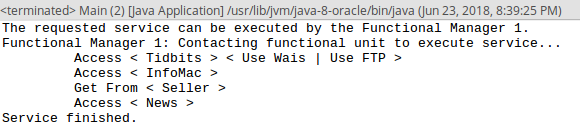
\includegraphics[scale=0.7]{figuras/macron/macron_console.png}
\caption{Saídas do console: \textit{FunctionalManager1Agent} executa o serviço solicitado.}
\label{fig:macron_console}
\end{figure}